\usetikzlibrary{patterns}%
\begin{figure}[htb]
\centering
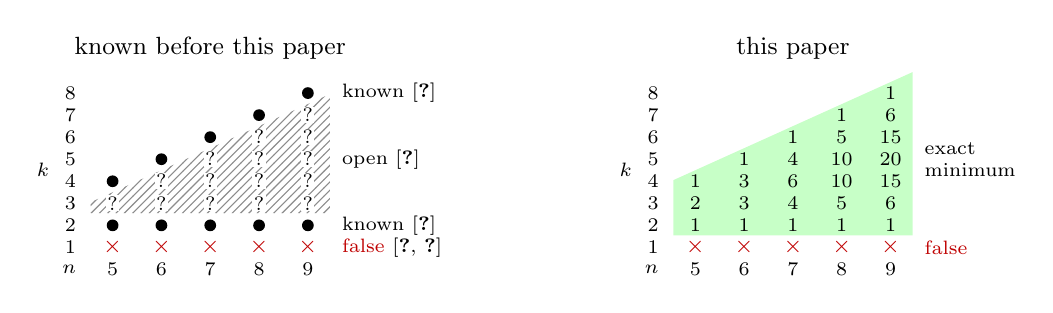
\begin{tikzpicture}[x=0.62cm,y=0.28cm,
  known/.style={circle,fill=black,inner sep=1.5pt},
  cross/.style={font=\footnotesize},
  num/.style={font=\scriptsize,inner sep=0.6pt}]
 \begin{scope}
  \fill[pattern=north east lines,pattern color=black!45]
    (-0.45,1.55) -- (4.45,1.55) -- (4.45,6.95) -- (-0.45,2.05) -- cycle;
  \foreach \n in {5,...,9} {
    \pgfmathtruncatemacro{\x}{\n-5}
    \node[cross,text=red!75!black] at (\x,0) {$\times$};
    \node[known] at (\x,1) {};
    \pgfmathtruncatemacro{\top}{\n-2}
    \node[known] at (\x,\top) {};
    \node[font=\scriptsize] at (\x,-1) {$\n$};
  }
  \foreach \n in {6,...,9} {
    \pgfmathtruncatemacro{\x}{\n-5}
    \pgfmathtruncatemacro{\last}{\n-2}
    \foreach \k in {3,...,\last} {
      \pgfmathtruncatemacro{\y}{\k-1}
      \node[font=\scriptsize,fill=white,inner sep=0.5pt] at (\x,\y) {?};
    }
  }
  \node[font=\scriptsize,fill=white,inner sep=0.5pt] at (0,2) {?};
  \foreach \k in {1,...,8} {\pgfmathtruncatemacro{\y}{\k-1}\node[font=\scriptsize,anchor=east] at (-0.55,\y) {$\k$};}
  \node[font=\scriptsize,anchor=east] at (-1.1,3.5) {$k$};
  \node[font=\scriptsize,anchor=east] at (-0.55,-1) {$n$};
  \node[font=\small,anchor=south] at (2,8.1) {known before this paper};
  \node[font=\scriptsize,anchor=west] at (4.5,0) {\textcolor{red!75!black}{false} \cite{HLSS,HL}};
  \node[font=\scriptsize,anchor=west] at (4.5,1) {known \cite{FLM}};
  \node[font=\scriptsize,anchor=west] at (4.5,7) {known \cite{HL}};
  \node[font=\scriptsize,anchor=west] at (4.5,4) {open \cite{Lee}};
 \end{scope}
 \begin{scope}[xshift=7.4cm]
  \fill[green!22] (-0.45,0.55) -- (4.45,0.55) -- (4.45,7.95) -- (-0.45,3.05) -- cycle;
  \foreach \n in {5,...,9} {
    \pgfmathtruncatemacro{\x}{\n-5}
    \node[cross,text=red!75!black] at (\x,0) {$\times$};
    \pgfmathtruncatemacro{\last}{\n-1}
    \foreach \k in {2,...,\last} {
      \pgfmathtruncatemacro{\y}{\k-1}
      \pgfmathtruncatemacro{\b}{round(factorial(\n-3)/(factorial(\k-2)*factorial(\n-1-\k)))}
      \node[num] at (\x,\y) {$\b$};
    }
    \node[font=\scriptsize] at (\x,-1) {$\n$};
  }
  \foreach \k in {1,...,8} {\pgfmathtruncatemacro{\y}{\k-1}\node[font=\scriptsize,anchor=east] at (-0.55,\y) {$\k$};}
  \node[font=\scriptsize,anchor=east] at (-1.1,3.5) {$k$};
  \node[font=\scriptsize,anchor=east] at (-0.55,-1) {$n$};
  \node[font=\small,anchor=south] at (2,8.1) {this paper};
  \node[font=\scriptsize,anchor=west] at (4.5,0) {\textcolor{red!75!black}{false}};
  \node[font=\scriptsize,anchor=west,align=left] at (4.5,4) {exact\\ minimum};
 \end{scope}
\end{tikzpicture}
\caption{The equality part of Conjecture~\ref{conj:HL} for posets with $n$ elements (columns) and faces of dimension $k$ (rows); for $n\leq4$ no poset contains $X$. Left, before this paper (sources in Table~\ref{tab:compare}): false for $k=1$ ($\times$), known for $k=2$ and for $k=n-1$ (dots), open otherwise (hatched, ?). Right, this paper: if $P$ contains $X$, then $\CC(P)$ has at least $\binom{n-3}{k-2}$ more $k$-dimensional faces than $\OO(P)$ (the number at each point), and one $n$-element poset attains all these bounds at once (Theorem~\ref{thm:main}); so, for $2\leq k\leq n-1$, equality holds exactly when $P$ does not contain $X$ (Corollary~\ref{cor:equality}). The second version of Fourier's preprint proves this equality statement independently \cite[Theorem~8.2]{FourierV2}, without an explicit lower bound.}\label{fig:beforeafter}
\end{figure}
